\renewcommand*{\arraystretch}{1.1}

\subsection*{Interactive / complex / 11}
\label{sec:interactive-complex-read-11}

\noindent\begin{tabularx}{\queryCardWidth}{|>{\queryPropertyCell}c|X|}
	\hline
	query & Interactive / complex / 11 \\ \hline
%
	title & Job referral \\ \hline
%
    pattern & \hfill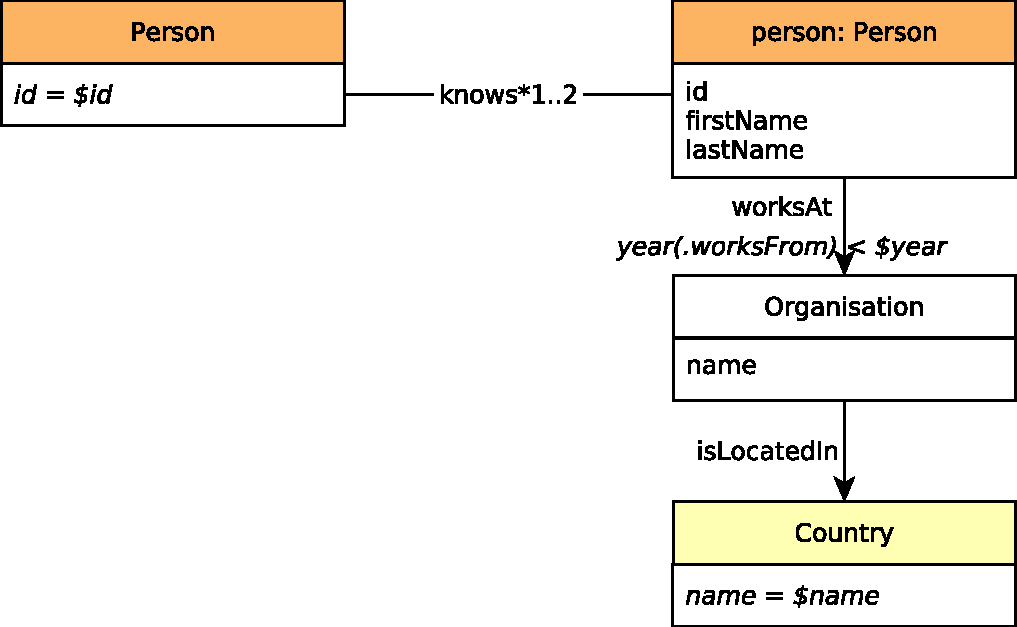
\includegraphics[scale=\patternscale,margin=0cm .2cm]{patterns/interactive-complex-read-11}\hfill\vadjust{} \\ \hline
%
	desc. & Given a start Person, find that Person's friends and friends of friends
(excluding start Person) who started Working in some Company in a given
Country, before a given date (year).
 \\ \hline
%
	
%
    
        params &
        \innerCardVSpace{\begin{tabularx}{\attributeCardWidth}{|>{\paramNumberCell}c|>{\varNameCell}M|>{\typeCell}m{\typeWidth}|Y|} \hline
        \cellcolor{parameter} \color{white} \footnotesize $\mathsf{1}$ &Person.id& ID &  \\ \hline
        \cellcolor{parameter} \color{white} \footnotesize $\mathsf{2}$ &Country.name& String &  \\ \hline
        \cellcolor{parameter} \color{white} \footnotesize $\mathsf{3}$ &year& 32-bit Integer &  \\ \hline
        \end{tabularx}}\innerCardVSpace \\ \hline
	
%
	
        result &
        \innerCardVSpace{\begin{tabularx}{\attributeCardWidth}{|>{\resultNumberCell}c|>{\varNameCell}M|>{\typeCell}m{\typeWidth}|>{\resultOriginCell}c|Y|} \hline
        $\mathsf{1}$ & Person.id & ID &R&
                 \\ \hline
        $\mathsf{2}$ & Person.firstName & String &R&
                 \\ \hline
        $\mathsf{3}$ & Person.lastName & String &R&
                 \\ \hline
        $\mathsf{4}$ & Person-worksAt->Organization.name & String &R&
                 \\ \hline
        $\mathsf{5}$ & Person-worksAt->.worksFrom & 32-bit Integer &R&
                 \\ \hline
        \end{tabularx}}\innerCardVSpace \\ \hline
	
%
	sort        &
        \innerCardVSpace{\begin{tabular}{|>{\sortNumberCell}c|>{\varNameCell}l|>{\directionCell}c|} \hline
        $\mathsf{1}$ & Person-worksAt->.worksFrom & $\asc$ \\ \hline
        $\mathsf{2}$ & Person.id & $\asc$ \\ \hline
        $\mathsf{3}$ & Person-worksAt->Organization.name & $\desc$ \\ \hline
        \end{tabular}}\innerCardVSpace \\ \hline
	%
	limit & 10 \\ \hline
	%
	CPs &
	\multicolumn{1}{>{\raggedright}l|}{
	    \chokePoint{1.4}, 
	    \chokePoint{2.3}, 
	    \chokePoint{2.4}, 
	    \chokePoint{3.3}
	    } \\ \hline
	%
    relevance &
        \small This query looks for paths of length two or three, starting from a Person, moving to friends or friends of friends,
and ending at a Company. In this query, there are selective joins and a top k order by that can be exploited for
optimizations.
 \\ \hline%
\end{tabularx}
\queryCardVSpace